% Figure s09f02_plasmon (Session 9): the particle-hole continuum and the plasmon.
% The image is rendered by figures/blender/s09f02_plasmon.py; the coordinates of the labels come from
% figures/blender/out/s09f02_plasmon*_anchors.tex. Build with figures/blender/build_figure.sh s09f02_plasmon.
\documentclass[11pt,tikz,border=0pt]{standalone}
\usepackage[T1]{fontenc}
\usepackage{amsmath,amssymb,graphicx,bm}
\usepackage{xcolor}
\usetikzlibrary{arrows.meta,calc}
% The three label colors of the figures, with the same values as in src/figures_preamble.tex.
\definecolor{aqmaccent}{RGB}{31,78,121}
\definecolor{aqmbroken}{RGB}{168,42,34}
\definecolor{aqmmuted}{RGB}{125,125,125}

% Shared TikZ styles of the overlays: axis arrows drawn on top of the renders, between anchors
% written by the scripts, so that they can be adjusted without rendering again.
\tikzset{
  axarrow/.style={line width=0.6pt, draw=black!70, -{Stealth[length=4.5pt,width=3.5pt]}},
  axlbl/.style={font=\small, inner sep=1.5pt},
}
% A discrete color key: \aqmkey{(x,y)}{color 1}{label 1}{color 2}{label 2} draws two swatches in a
% column with their labels, anchored at its north west corner. The colors are the sRGB values
% used in the render, defined below.
\definecolor{keypos}{RGB}{118,158,198}
\definecolor{keyneg}{RGB}{214,150,132}
\definecolor{keyup}{RGB}{224,62,40}
\definecolor{keydown}{RGB}{40,92,200}
\definecolor{keydark}{RGB}{31,78,121}
\definecolor{keylight}{RGB}{118,158,198}
\newcommand{\aqmkey}[5]{%
  \begin{scope}[shift={#1}]
    \fill[#2, draw=black!40, line width=0.3pt] (0,-0.32) rectangle (0.32,0);
    \node[font=\small, anchor=west, inner sep=1.5pt] at (0.38,-0.16) {#3};
    \fill[#4, draw=black!40, line width=0.3pt] (0,-0.74) rectangle (0.32,-0.42);
    \node[font=\small, anchor=west, inner sep=1.5pt] at (0.38,-0.58) {#5};
  \end{scope}}
% The same key in one row, for a figure with no room for a column.
\newcommand{\aqmkeyrow}[5]{%
  \begin{scope}[shift={#1}]
    \fill[#2, draw=black!40, line width=0.3pt] (0,-0.32) rectangle (0.32,0);
    \node[font=\small, anchor=west, inner sep=1.5pt] (k1) at (0.38,-0.16) {#3};
    \fill[#4, draw=black!40, line width=0.3pt] ([xshift=0.25cm]k1.east |- 0,-0.32) rectangle ++(0.32,0.32);
    \node[font=\small, anchor=west, inner sep=1.5pt] at ([xshift=0.63cm]k1.east) {#5};
  \end{scope}}

\newlength{\figw}\setlength{\figw}{10.10cm}   % 0.65 of the text width, before the empty margins of the render are cropped

\begin{document}
\begin{tikzpicture}[lbl/.style={font=\small, inner sep=1.5pt}, pnl/.style={font=\small\bfseries, inner sep=1.5pt}]
  \begin{scope}[shift={(0.00cm,0.00cm)}]
    \setlength{\figw}{10.10cm}
    \node[overlay, anchor=south west, inner sep=0pt] at (0,0)
      {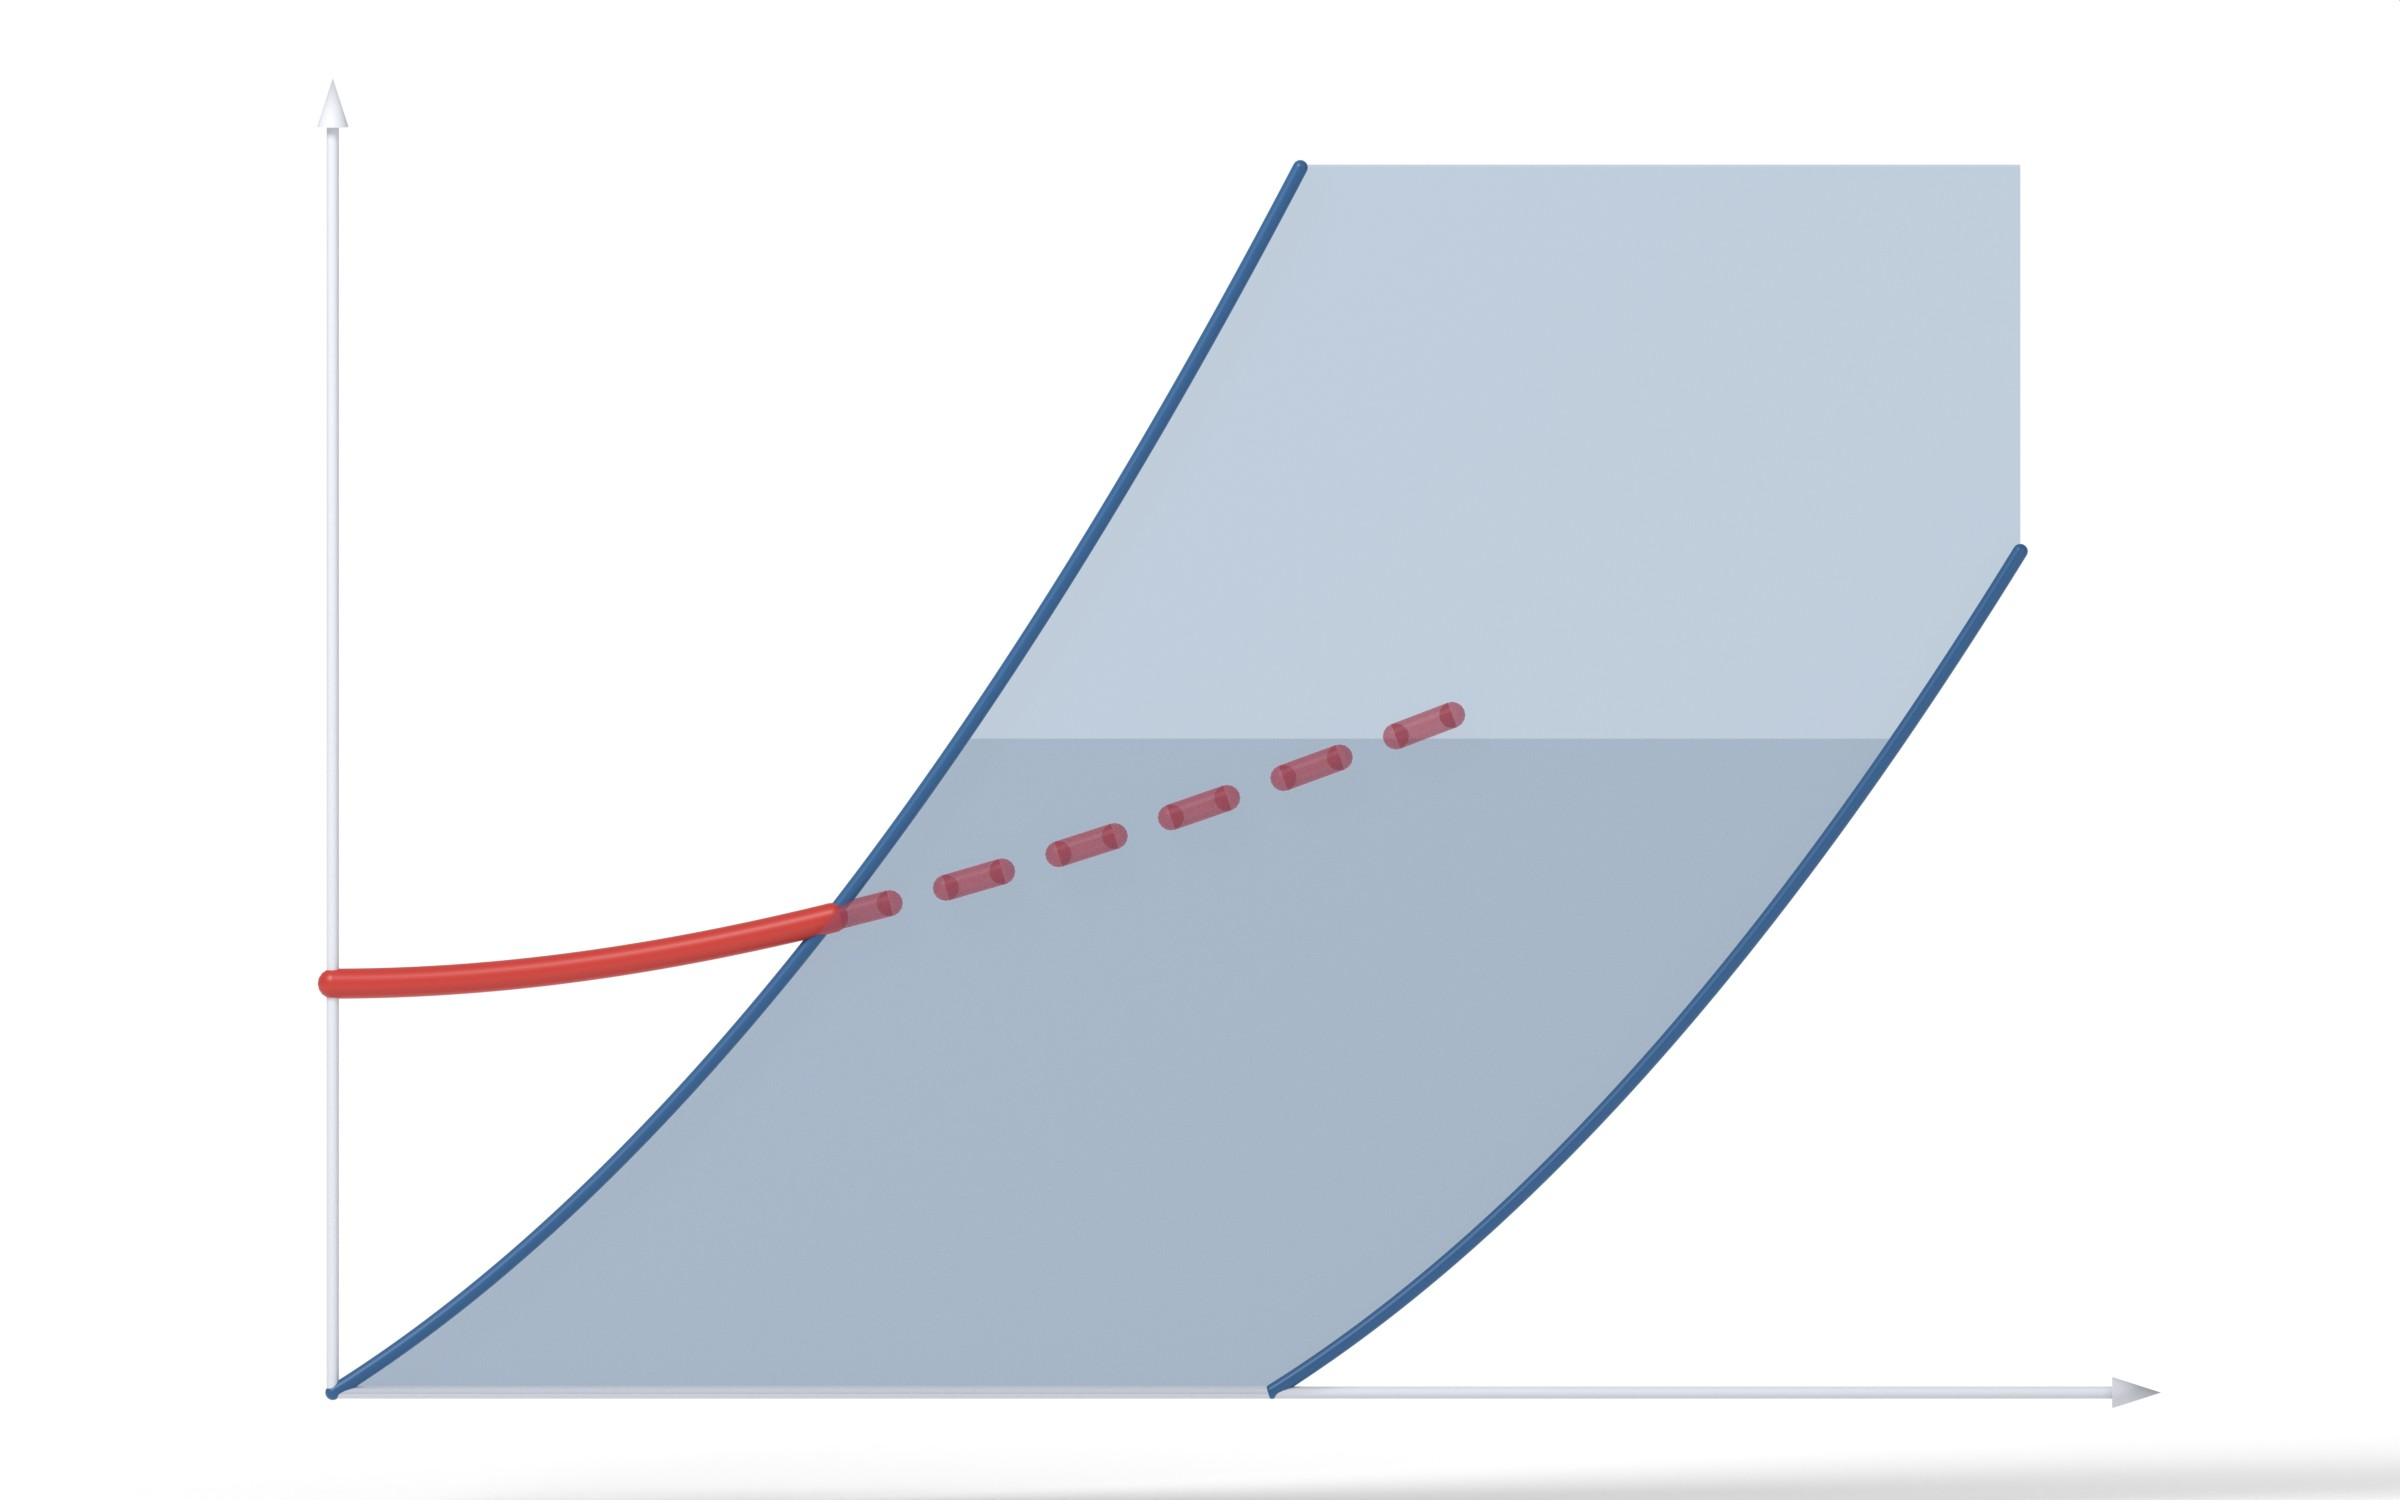
\includegraphics[width=\figw]{../blender/out/s09f02_plasmon.jpg}};
    % written by build_figure.sh; the painted part of the image
\path (0.1321\figw,0.0013\figw) rectangle (0.9988\figw,0.5925\figw);

    %% written by figlib.py; x and y in units of the image width
\coordinate (q) at (0.9004\figw,0.0447\figw);
\coordinate (w) at (0.1387\figw,0.5924\figw);
\coordinate (wp) at (0.1387\figw,0.2151\figw);
\coordinate (twokf) at (0.5293\figw,0.0447\figw);
\coordinate (plasmon) at (0.1875\figw,0.2228\figw);
\coordinate (cont) at (0.6074\figw,0.2395\figw);
\coordinate (window) at (0.1543\figw,0.3794\figw);
\coordinate (damped) at (0.5914\figw,0.3097\figw);

    \node[lbl, anchor=north east] at (q) {$q/k_F$};
    \node[lbl, anchor=west] at (w) {$\omega$};
    \node[lbl, anchor=east, text=aqmbroken] at (wp) {$\omega_p$};
    \node[lbl, anchor=north] at (twokf) {$2$};
    \node[lbl, anchor=south west, xshift=-6pt, text=aqmbroken] at (plasmon) {plasmon};
    \node[lbl, anchor=west, text=aqmaccent] at (cont) {continuum};
    \node[lbl, anchor=west, text=aqmmuted, align=left] at (window) {no particle-hole\\pairs here};
    \node[lbl, anchor=south, yshift=2pt, text=aqmbroken] at (damped) {Landau damped};
  \end{scope}
\end{tikzpicture}
\end{document}
